\documentclass[../report.tex]{subfiles}

\begin{document}

Aan het begin van het project is een ontwerp gemaakt van hoe het project eruit zou kunnen zien. In dit hoofdstuk wordt het ontwerp van het project besproken en wordt er uitgelegd waarom bepaalde keuzes zijn gemaakt.

\section{Architectuur}

Er zijn drie programma's bedacht om het project te realiseren:

\begin{itemize}
  \item \collector{}: Een programma dat specificaties verzamelt en verstuurt.
  \item \server{}: Een \gls*{API} voor het opslaan en ophalen van de specificaties.
  \item \dashboard{}: Een webapplicatie voor het weergeven van de specificaties.
\end{itemize}

De oorspronkelijke lijst van specificaties die door de collector verstuurd moet worden is te vinden in een apart document \parencite{specificaties}.

Deze programma's werken samen zoals omschreven in \autoref{fig:architecture}. In het diagram is te zien hoe de collector draaiend op een aantal bare-metal \glspl*{server} en VMs gegevens versturen naar de \gls*{API}. Dit programma slaat de gegevens op in de database. De webapplicatie (te vinden in de micro-frontends monorepo) haalt de gegevens op uit de \gls*{API} en toont deze aan de gebruiker.

\begin{figure}
  \centering
  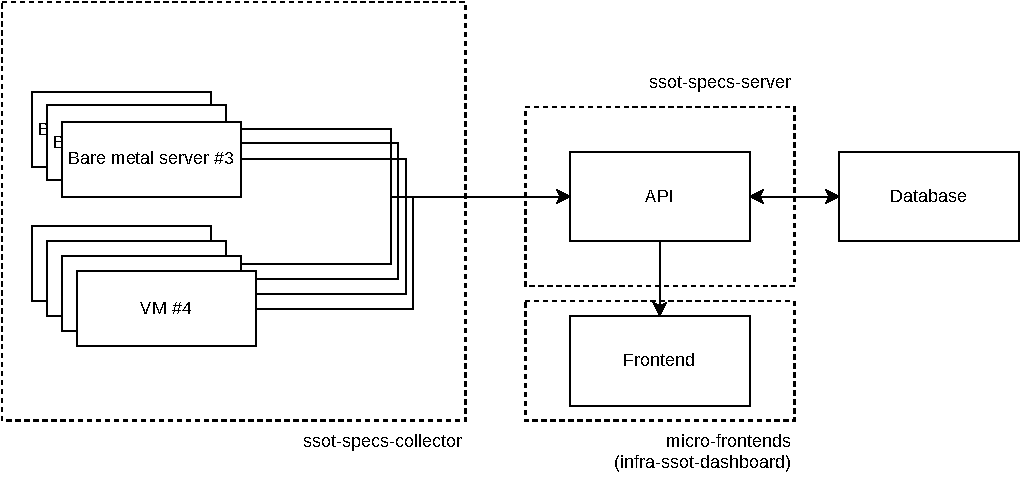
\includegraphics[width=0.85\textwidth]{../assets/images/drawio/architecture.pdf}
  \caption{Overzicht van de architectuur van de \gls*{SSOT}. Een pijl geeft de richting van de gegevensstroom aan, een rechthoek is een programma en een gestippelde rechthoek is een inkapseling van een beroepsproduct.}
  \label{fig:architecture}
\end{figure}

\section{Alternatieven}
\label{sec:alternatieven}

Voordat de ontwikkeling begon is ook nagedacht om NetBox te gebruiken. De \gls*{product owner} had aangeraden om onderzoek te doen naar welke software reeds bestaat om het product mee te realiseren, en had zelf NetBox als suggestie meegegeven.

NetBox leek echter niet geschikt voor het project. NetBox is gemaakt voor het beheren van netwerkapparatuur, en bevat daardoor veel functionaliteiten voor dit specifieke doel. Bovendien zijn er veel onnodige functionaliteiten, zoals verplichte categorieën die niet relevant zijn voor het gewenste product. NetBox ondersteunt verder geen componenten zoals geheugen of opslag van een apparaat, maar het is wel mogelijk om \textit{custom fields} te maken \parencite{netbox_custom_fields}. Tenslotte was het niet duidelijk of apparaten overschreven konden worden. Achteraf gezien had er meer tijd aan het onderzoek naar het gebruik van NetBox besteed kunnen worden, zodat het misschien toch gebruikt had kunnen worden.

Om de data op te slaan is een database nodig zoals vermeld in \autoref{fig:architecture}. Voor deze database is een ontwerp gemaakt. Er waren twee mogelijkheden: de database specifiek of algemeen ontwerpen. Hiermee wordt bedoeld of er aparte, van tevoren gedefinieerde tabellen moesten zijn per specificatie (niet te verwarren met de \gls*{OpenAPI-specificatie}), of dat de specificaties in rijen konden worden gedefinieerd. Het voordeel van een algemene database is dat het gemakkelijk is om specificaties toe te voegen, maar het nadeel is dat er per ongeluk oude, ongebruikte of anderzijds verkeerde data in voor kunnen komen van specificaties die niet meer gebruikt worden. De \gls*{product owner} had aangegeven voorkeur te hebben voor de specifieke database gezien deze argumenten. Het algemene ontwerp is wel bewaard en is te vinden in \autoref{fig:erd}.

\begin{figure}
  \centering
  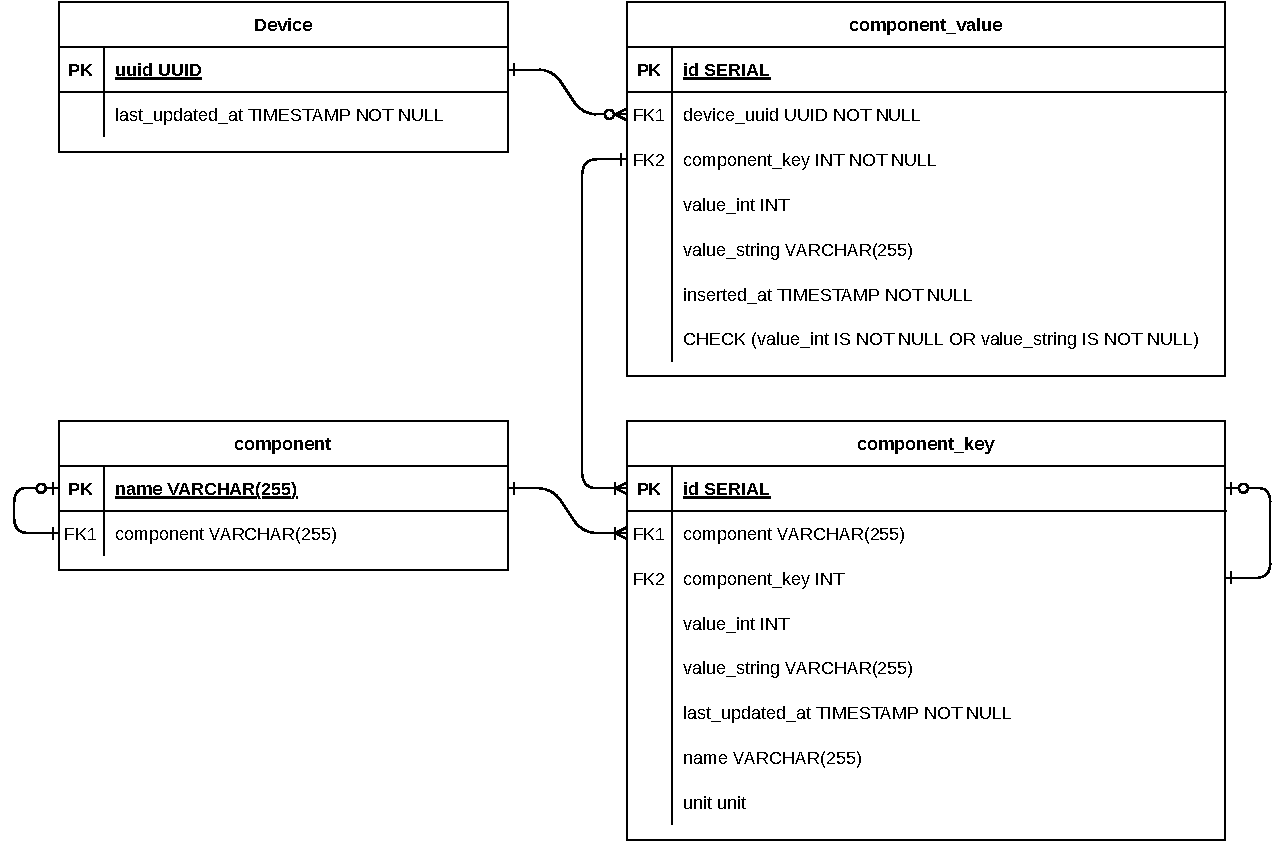
\includegraphics[width=0.85\textwidth]{../assets/images/drawio/erd.pdf}
  \caption{Ontwerp \gls*{ERD} voor algemene database.}
  \label{fig:erd}
\end{figure}

\end{document}
